\documentclass[12pt]{article}
\usepackage{amsmath}
\usepackage{amssymb}
\usepackage{geometry}
\usepackage{amsmath, amsfonts, bm, graphicx}
\usepackage{tabularx}
\usepackage{booktabs} 
\usepackage{float}
\usepackage{enumitem}
\geometry{margin=1in}

\title{}
\date{}
\author{}

\begin{document}
\subsection*{\boxed{\text{HW 4 - Zeshui Song}}}

\section*{5.25}
\vspace{-2em}
\begin{center}
    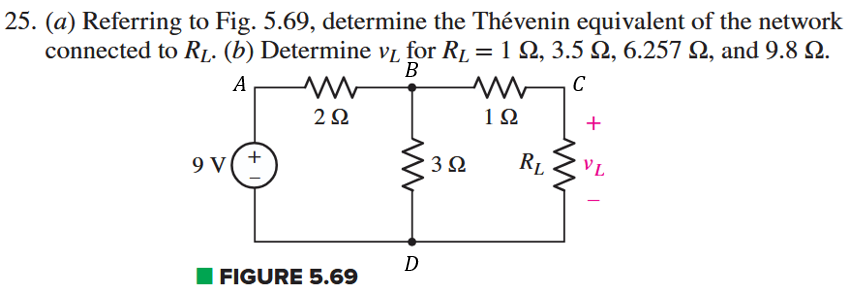
\includegraphics[width=0.8\textwidth]{5-25.png}
\end{center}
\vspace{-1em}
\textbf{(a)} Finding the Thevenin equivalent. Starting with finding the open circuit voltage $V_{oc}$ across the load resistor $R_L$ (remove $R_L$ from the circuit):
\begin{center}
    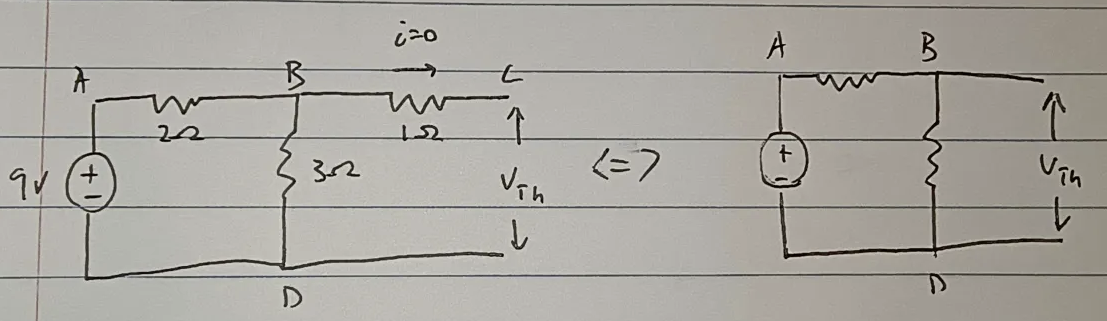
\includegraphics[width=0.8\textwidth]{5-25_1.png}
\end{center}
Thus, $V_{oc}$ is the same voltage across nodes B and D. Using voltage division:
\[V_{BD} = V_{oc} = \frac{[3\,\Omega]}{[2+3\,\Omega]} [9\,\text{V}] = 5.4\,\text{V} \]
To find the Thevenin equivalent resistance $R_{Th}$, we turn off all independent sources (replace voltage sources with \textbf{short circuits} and current sources with \textbf{open circuits}) and find the equivalent resistance across nodes C and D:
\begin{center}
    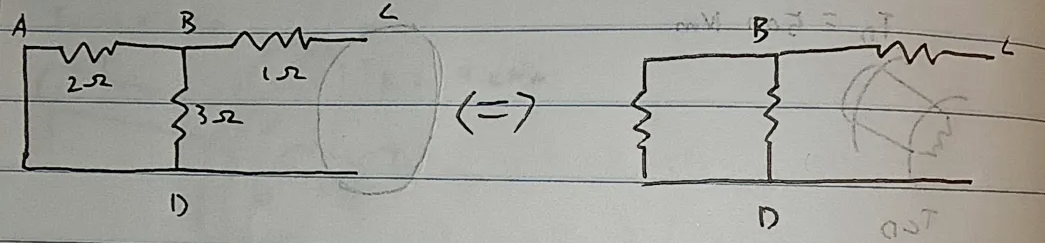
\includegraphics[width=0.8\textwidth]{5-25_2.png}
\end{center}
Add the parallel resistors $2\Omega + 3\Omega$:
\[R = \frac{[2\cdot3\Omega]}{[2+3\Omega]} = 1.2\,\Omega\]
Add the series resistor $1\Omega$:
\[R_{Th} = 1\Omega + 1.2\Omega = 2.2\Omega\]
Thus:
\[\boxed{V_{Th} = V_{oc} = 5.4\,\text{V}\quad R_{Th} = 2.2\Omega}\]
\newpage\noindent
\textbf{(b)} Using the Thevenin equivalent circuit, we can use voltage division to find the voltage across the load resistor $R_L$:
\begin{center}
    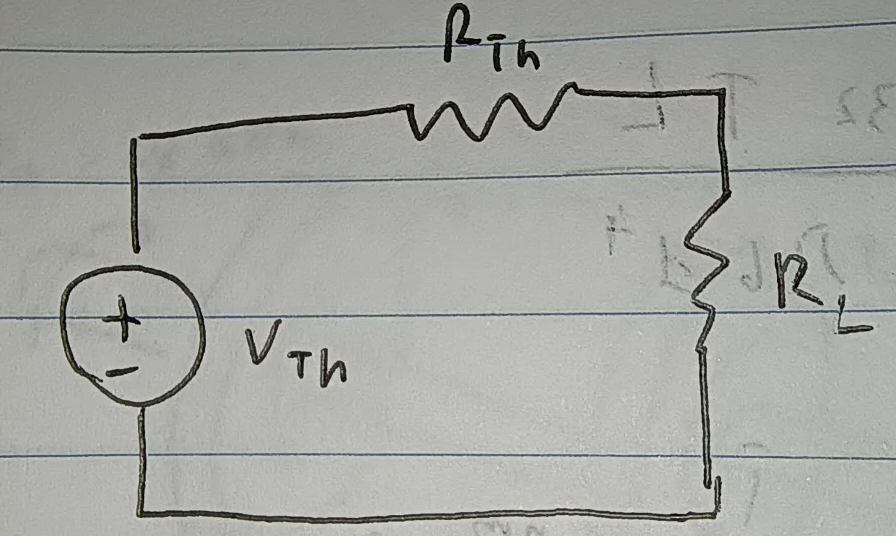
\includegraphics[width=0.4\textwidth]{5-25_3.png}
\end{center}
\begin{itemize}
    \item $R_L = 1\Omega$: \[V_L = \frac{[1\Omega]}{[2.2\Omega + 1\Omega]} [5.4\,\text{V}] = 1.687\,\text{V}\]
    \item $R_L = 3.5\Omega$: \[V_L = \frac{[3.5\Omega]}{[2.2\Omega + 3.5\Omega]} [5.4\,\text{V}] = 3.315\,\text{V}\]
    \item $R_L = 6.257\Omega$: \[V_L = \frac{[6.257\Omega]}{[2.2\Omega + 6.257\Omega]} [5.4\,\text{V}] = 3.995\,\text{V}\]
    \item $R_L = 9.8\Omega$: \[V_L = \frac{[9.8\Omega]}{[2.2\Omega + 9.8\Omega]} [5.4\,\text{V}] = 4.41\,\text{V}\]
\end{itemize}

\section*{5.30}
\vspace{-2em}
\begin{center}
    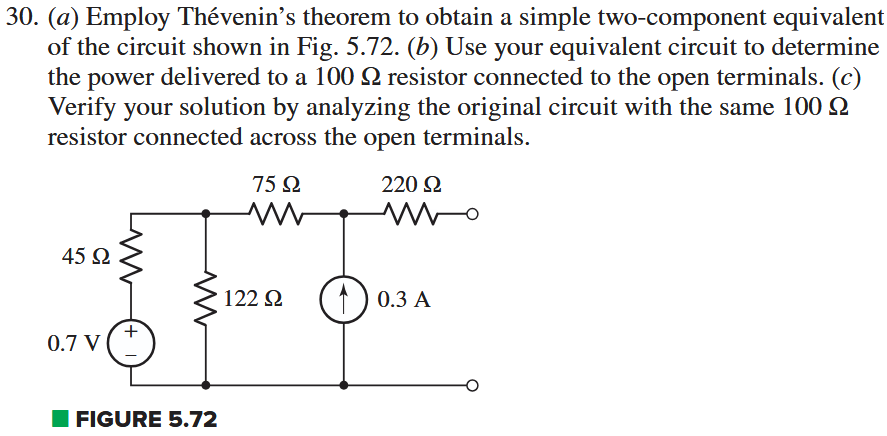
\includegraphics[width=0.8\textwidth]{5-30.png}
\end{center}
\vspace{-1em}
\textbf{(a)} Finding the Thevenin equivalent. Starting with finding the open circuit voltage $V_{oc}$ by using nodal analysis. Like before, there is no current flowing through the 220$\Omega$ resistor, so the voltage across the current source is equal to $V_{oc}$:
\begin{center}
    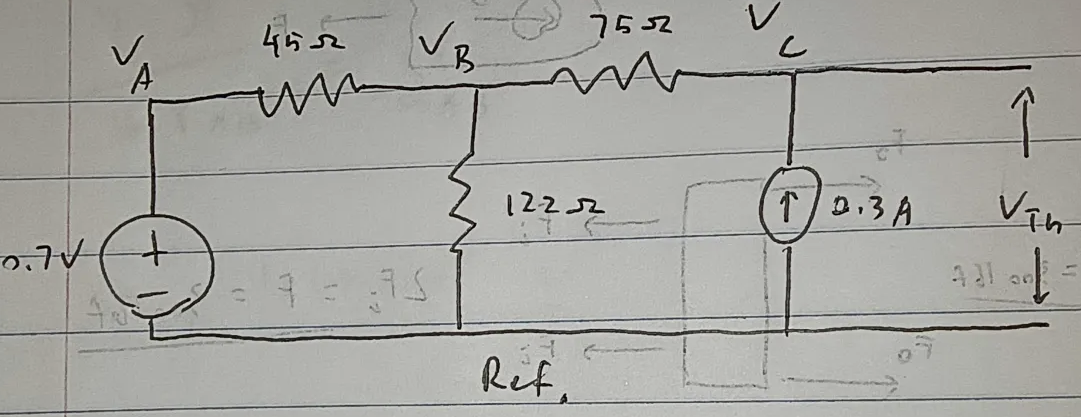
\includegraphics[width=0.8\textwidth]{5-30_1.png}
\end{center}
Node A:
\[V_A = 0.7\,\text{V}\]
KCL at node B:
\[\frac{[V_A - V_B]}{[45\,\Omega]} = \frac{V_B}{122\,\Omega}+\frac{V_B-V_C}{75\,\Omega} \quad \implies \quad 0.0437522V_B-0.0133333V_C = 0.015555\]
KCL at node C:
\[\frac{V_B-V_C}{75\,\Omega} = -0.3\,\text{A}\quad \implies \quad 0.0133333V_B-0.0133333V_C = -0.3\]
Thus, $V_B = 10.373\,\text{V}$ and $V_C = 32.873\,\text{V}$. Therefore, $\boxed{V_{oc} = V_C=32.873\,\text{V}}$.\\\\
To find the Thevenin equivalent resistance $R_{Th}$, we turn off all independent sources:
\begin{center}
    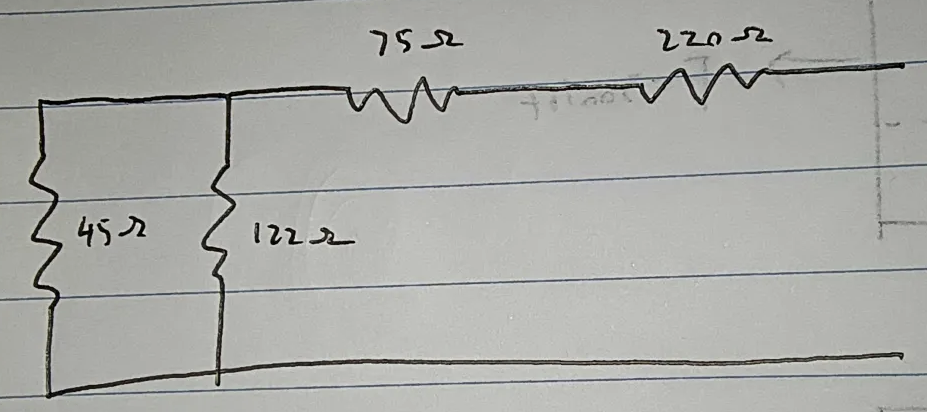
\includegraphics[width=0.5\textwidth]{5-30_2.png}
\end{center}
Combine the parallel resistors $45\Omega$ and $122\Omega$:
\[R = \frac{[45\cdot122\,\Omega]}{[45+122\Omega]} = 33.87\,\Omega\]
Add to the series resistors $75\Omega$ and $220\Omega$:
\[\boxed{R_{Th} = 33.87\Omega + 75\Omega + 220\Omega = 327.87\,\Omega}\]
\textbf{(b)} Power delivered to the load resistor $R_L=100\Omega$. First find the voltage across $R_L$ using voltage division:
\[V_L = \frac{[100\,\Omega]}{100+327.87\,\Omega} [32.873\,\text{V}] = 7.682\,\text{V}\]
Thus the power delivered to $R_L$ is:
\[P_L = \frac{V_L^2}{R_L} = \frac{[7.682\,\text{V}]^2}{[100\,\Omega]} = \boxed{0.59\,\text{W}}\]
\textbf{(c)} We can apply nodal analysis to the circuit including the 100$\Omega$ load resistor to find the voltage across $R_L$. 
\begin{center}
    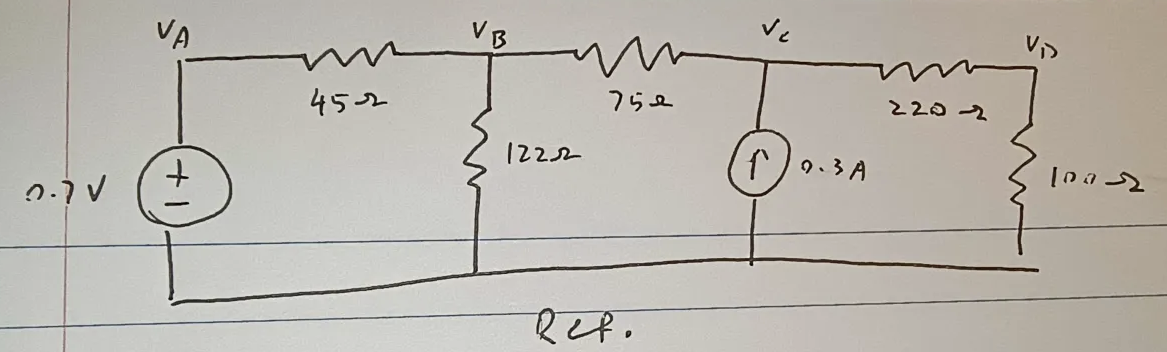
\includegraphics[width=0.8\textwidth]{5-30_3.png}
\end{center}
Node A:
\[V_A = 0.7\,\text{V}\]
KCL at node B:
\[\frac{[V_A - V_B]}{[45\,\Omega]} = \frac{V_B}{122\,\Omega}+\frac{V_B-V_C}{75\,\Omega} \quad \implies \quad 0.0437522V_B-0.0133333V_C = 0.015555\]
KCL at node C:
\[\frac{V_B-V_C}{75\,\Omega} = [-0.3\,\text{A}] + \frac{V_C-V_D}{220\,\Omega} \quad \implies \quad 0.0133333V_B-0.017878V_C+0.004545V_D = -0.3\]
KCL at node D:
\[\frac{V_C-V_D}{220\,\Omega} = \frac{V_D}{100\,\Omega} \quad \implies \quad 0.004545V_C-0.01454545V_D = 0\]
Thus, $V_B = 7.848\,\text{V}$, $V_C = 24.586\,\text{V}$, and $V_D = V_L = 7.682\,\text{V}$. 
Thus the power delivered to $R_L$ is:
\[P_L = \frac{V_L^2}{R_L} = \frac{[7.682\,\text{V}]^2}{[100\,\Omega]} = \boxed{0.59\,\text{W}}\]
\newpage

\section*{5.32}
\vspace{-2em}
\begin{center}
    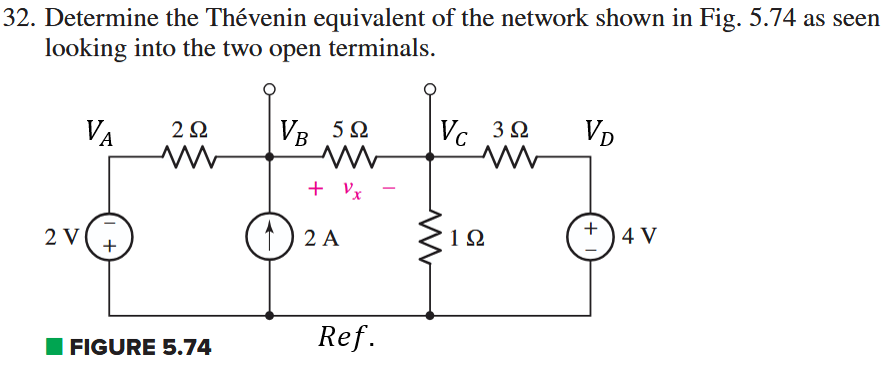
\includegraphics[width=0.8\textwidth]{5-32.png}
\end{center}
\vspace{-1em}
The open circuit voltage $V_{oc} = V_B - V_C$. Using nodal analysis:\\\\
Node A:
\[V_A = -2\,\text{V}\]
KCL at node B:
\[\frac{V_A - V_B}{[2\,\Omega]} = \frac{V_B-V_C}{[5\,\Omega]} - [2\,\text{A}]\quad\implies\quad 0.5V_A - 0.7V_B + 0.2V_C = -2\]
KCL at node C:
\[\frac{V_B-V_C}{[5\,\Omega]} = \frac{V_C}{[1\,\Omega]} + \frac{V_C-V_D}{[3\,\Omega]}\quad\implies\quad 0.2V_B - 1.5333V_C + 0.333V_D = 0\]
Node D:
\[V_D = 4\,\text{V}\]
Thus, $V_B = 1.741\,\text{V}$ and $V_C = 1.096\,\text{V}$. Therefore, $\boxed{V_{oc} = V_B - V_C = 0.645\,\text{V}}$.\\\\
Finding the Thevenin equivalent resistance $R_{Th}$, we turn off all independent sources:
\begin{center}
    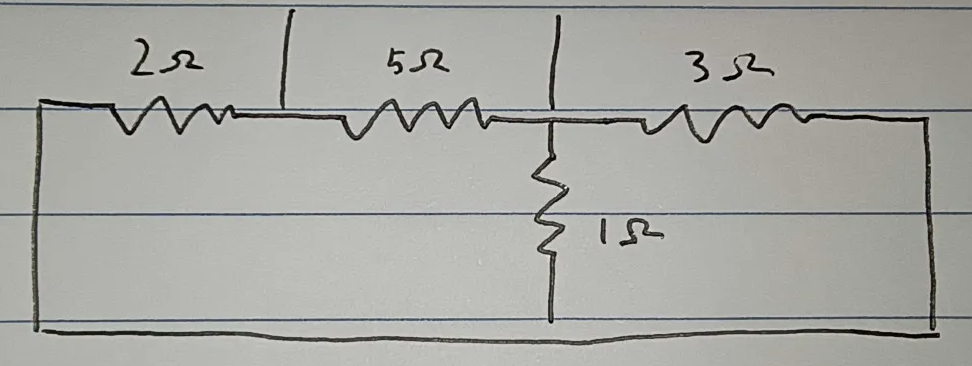
\includegraphics[width=0.5\textwidth]{5-32_1.png}
\end{center}
\begin{minipage}[t]{0.5\textwidth}\vspace{0pt}
Combine the parallel resistors $1\Omega + 3\Omega$:
\[R = \frac{[1\cdot3\,\Omega]}{[1+3\,\Omega]} = 0.75\,\Omega\]
\end{minipage}
\hfill
\begin{minipage}[t]{0.5\textwidth}\vspace{0pt}
\centering
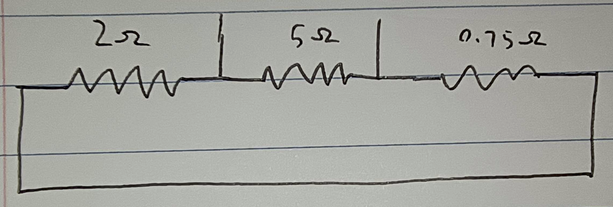
\includegraphics[width=\textwidth]{5-32_2.png}
\end{minipage}\\
\begin{minipage}[t]{0.5\textwidth}\vspace{0pt}
Combine 2$\Omega$ and 0.75$\Omega$ in series:
\[R = 2\,\Omega + 0.75\,\Omega = 2.75\,\Omega\]
Finally, combine 2.75$\Omega$ and 5$\Omega$ in parallel:
\[\boxed{R_{Th} = \frac{[2.75\cdot5\,\Omega]}{[2.75+5\,\Omega]} = 1.774\,\Omega}\]
\end{minipage}
\hfill
\begin{minipage}[t]{0.5\textwidth}\vspace{0pt}
\centering
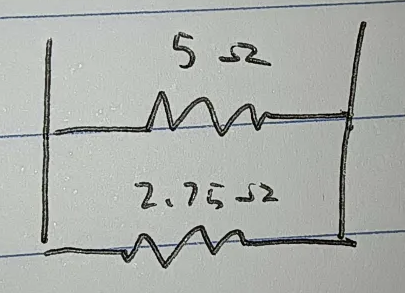
\includegraphics[width=0.6\textwidth]{5-32_3.png}
\end{minipage}

\section*{5.40}
\vspace{-2em}
\begin{center}
    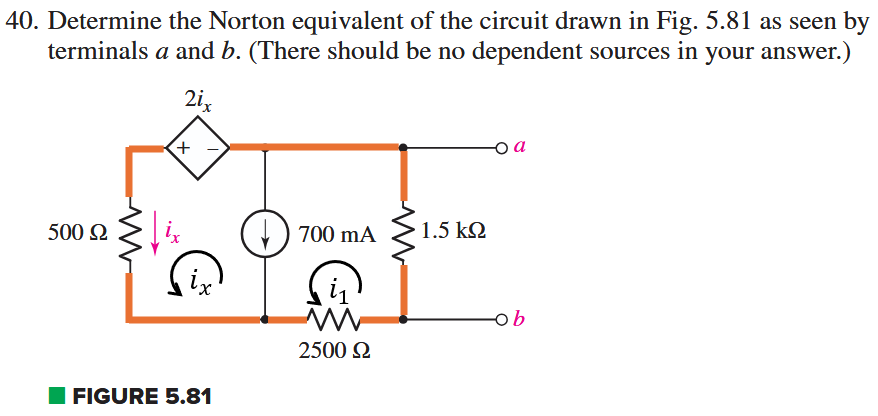
\includegraphics[width=0.8\textwidth]{5-40.png}
\end{center}
\vspace{-1em}
The \textit{Norton equivalent} circuit is the same as the Thevenin equivalent circuit, except the voltage source is transformed into a current source. However, since there is a dependent voltage source in the circuit, we cannot directly find the Thevenin equivalent resistance by turning off all independent sources and summing up the resistances. Instead, we define a short circuit current $i_{sc}=i_N$ by shorting the terminals of the load (place a wire across it). Then, the two circuits are related by a source transformation:
\[\boxed{V_{Th} = R_{Th} i_{N}}\]
\[\boxed{R_{Th} = R_{N}}\]
\underline{Note:} If the dependent source is controlled by the load voltage, shorting it would cause this voltage to be zero and thus the dependent source would be turned off.\\\\
First, using mesh analysis, we can find the current $i_1$ passing through the 1.5 k$\Omega$ resistor and thus find the open circuit voltage $V_{oc}$.\\\\
KVL around the orange supermesh:
\[(2i_x)-[500\,\Omega]i_x-[2500\,\Omega]i_1 -[1500\,\Omega]i_1 = 0\quad\implies\quad -4000i_1 -498i_x = 0\]
Supermesh equation:
\[i_1 - i_x = 700\times10^{-3}\,\text{A}\]
Thus, $i_1 = 0.0775\,\text{A}$ and $i_x = -0.6224\,\text{A}$. Therefore, the open circuit voltage is:
\[V_{oc} = [1.5\,\text{k}\Omega]i_1 = \boxed{116.25\,\text{V}}\]
Next, we find the short-circuit current $i_{sc}$. When the terminals of the load resistor are shorted, we can again apply mesh analysis. The short creates a path with essentially zero resistance in parallel with the $1.5\,\text{k}\Omega$ resistor, so the current flows through the short instead. As a result, no current passes through the $1.5\,\text{k}\Omega$ resistor.
\begin{center}
    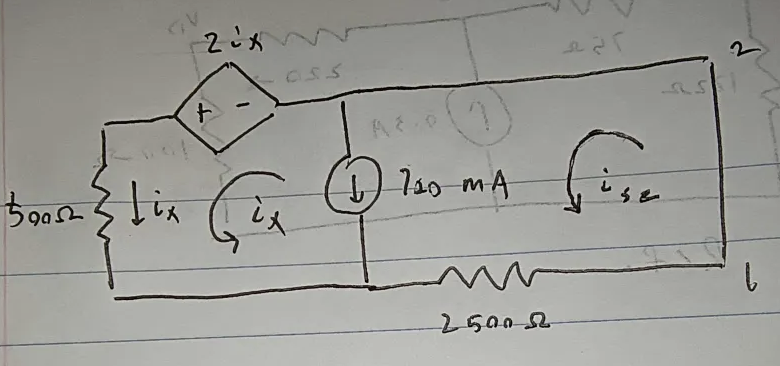
\includegraphics[width=0.8\textwidth]{5-40_1.png}
\end{center}
KVL around the supermesh:
\[(2i_x)-[500\,\Omega]i_x-[2500\,\Omega]i_{sc} = 0\quad\implies\quad -498i_x - 2500i_{sc} = 0\]
Supermesh equation:
\[i_{sc} - i_x = 700\times10^{-3}\,\text{A}\]
Thus, $i_{sc} = 0.1162\,\text{A}$ and $i_x = -0.5837\,\text{A}$. \\\\
Finally, we can find the Thevenin equivalent resistance:
\[R_{Th} = \frac{V_{oc}}{i_{sc}} = \frac{[116.25\,\text{V}]}{[0.1162\,\text{A}]}= \boxed{1000.43\,\Omega}\]
The Norton equivalent is then:
\[\boxed{i_N = i_{sc} = 0.1162\,\text{A}, \quad R_N = R_{Th} = 1000.43\,\Omega}\]
\begin{center}
    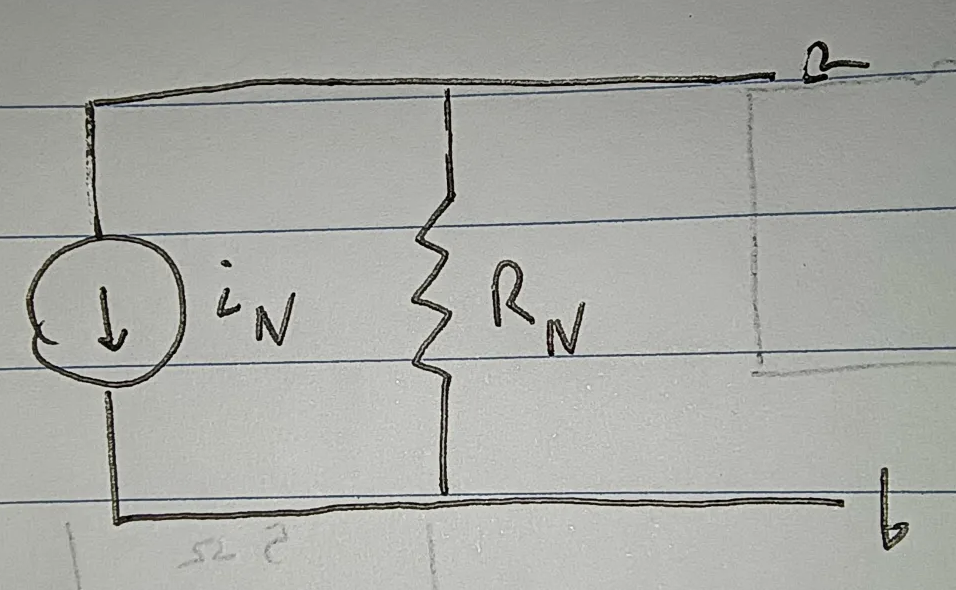
\includegraphics[width=0.4\textwidth]{5-40_2.png}
\end{center}

\section*{5.44}
\vspace{-2em}
\begin{center}
    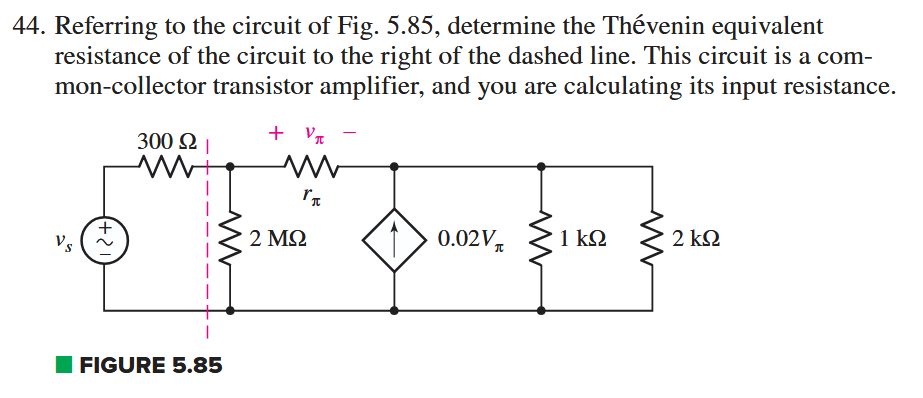
\includegraphics[width=0.8\textwidth]{5-44.png}
\end{center}
\vspace{-1em}
For this circuit, the dependent current source means that we cannot sum up the resistances to find the Thevenin equivalent resistance. We can either find the open circuit voltage $V_{oc}$ and short circuit current $i_{sc}$ or we can apply a test voltage source $V_{Test}$ across the load terminals and find the resulting current $i_{Test}$ to find the Thevenin equivalent resistance.\\\\
Note that because there are no \textit{independent sources} in the circuit, both the open circuit voltage $V_{oc}$ and short circuit current $i_{sc}$ are zero. Thus, we cannot find the Thevenin equivalent resistance using the first method. So, we will use the test source method (turning off all independent sources to see the circuit's response; there are no independent sources in this case).\\\\
We can simplify the 1 k$\Omega$ and 2 k$\Omega$ resistors in parallel. 
\[R=\frac{[1\cdot2\,\text{k}\Omega]}{[1+2\,\text{k}\Omega]} = 0.666\,\text{k}\Omega\]
\begin{center}
    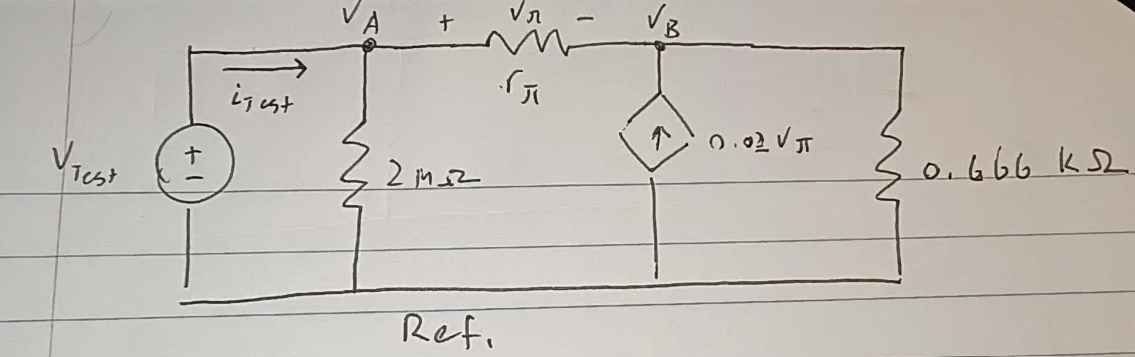
\includegraphics[width=0.8\textwidth]{5-44_1.png}
\end{center}
\[V_{\pi} = V_A - V_B\]
\[V_\text{Test}=V_A\]
KCL at node A:
\[i_\text{Test}=\frac{V_A}{[2000\,\text{k}\Omega]} + \frac{V_A-V_B}{r_{\pi}}\]
KCL at node B:
\[\frac{V_A-V_B}{r_{\pi}} = [-0.02V_{\pi}]+\frac{V_B}{[0.666\,\text{k}\Omega]}\quad\implies\quad\frac{V_A-V_B}{r_{\pi}} = [-0.02(V_A - V_B)]+\frac{V_B}{[0.666\,\text{k}\Omega]}\]
\[V_A\left(0.02+\frac{1}{r_{\pi}}\right) + V_B\left(-\frac{1}{r_{\pi}} -0.02-\frac{1}{0.666}\right) = 0\]
\[V_B = V_A \frac{\left(0.02+\frac{1}{r_{\pi}}\right)}{\left(\frac{1}{r_{\pi}} +0.02+\frac{3}{2}\right)}\]
Plug this into the equation for $i_\text{Test}$ to find the ratio $R_{Th} = \frac{V_\text{Test}}{i_\text{Test}} = \frac{V_A}{i_\text{Test}}$:
\[i_\text{Test}=V_A\left(\frac{1}{[2000\,\text{k}\Omega]}+\frac{1}{r_{\pi}}\right) - \frac{1}{r_{\pi}}\left[V_A \frac{\left(0.02+\frac{1}{r_{\pi}}\right)}{\left(\frac{1}{r_{\pi}} +0.02+\frac{3}{2}\right)}\right]\]
\[\frac{1}{R_{Th}} = \frac{i_\text{Test}}{V_A} = \left(\frac{1}{2000}+\frac{1}{r_{\pi}}\right) - \frac{1}{r_{\pi}}\left[\frac{\left(0.02+\frac{1}{r_{\pi}}\right)}{\left(\frac{1}{r_{\pi}} +0.02+\frac{3}{2}\right)}\right]\]
\[\boxed{R_{Th} = \left[\left(\frac{1}{2000}+\frac{1}{r_{\pi}}\right) - \frac{1}{r_{\pi}}\left[\frac{\left(0.02+\frac{1}{r_{\pi}}\right)}{\left(\frac{1}{r_{\pi}} +0.02+\frac{3}{2}\right)}\right]\right]^{-1}}\]

\section*{5.51}
\vspace{-2em}
\begin{center}
    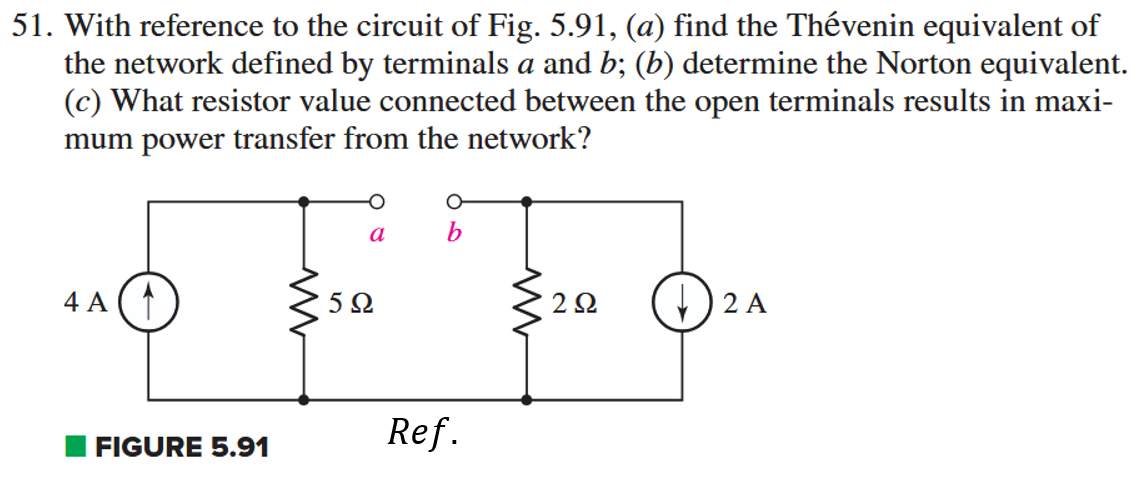
\includegraphics[width=0.8\textwidth]{5-51.png}
\end{center}
\vspace{-1em}
\textbf{(a)} Start by finding the open circuit voltage $V_{oc}$ across nodes a and b, keeping track of polarity.
\[V_a = [5\,\Omega][4\,\text{A}] = 20\,\text{V}\]
\[V_b = [2\,\Omega][-2\,\text{A}] = -4\,\text{V}\]
\[V_{Th}=V_{oc} = V_a - V_b = 20\,\text{V} - (-4\,\text{V}) = \boxed{24\,\text{V}}\]
The Thevenin equivalent resistance after turning off the independent sources is:
\[\boxed{R_{Th} = 5\,\Omega + 2\,\Omega = 7\,\Omega}\]
\textbf{(b)} Using the Thevenin equivalent, we just source transform to find the Norton equivalent:
\[\boxed{i_N = \frac{V_{Th}}{R_{Th}} = \frac{24\,\text{V}}{7\,\Omega} = 3.428\,\text{A}, \quad R_N = R_{Th} = 7\,\Omega}\]
\textbf{(c)} The maximum power transfer occurs when the load resistance $R_L$ is equal to the Thevenin equivalent resistance $R_{Th}$:
\[\boxed{R_L = R_{Th} = 7\,\Omega}\]

\section*{5.53}
\vspace{-2em}
\begin{center}
    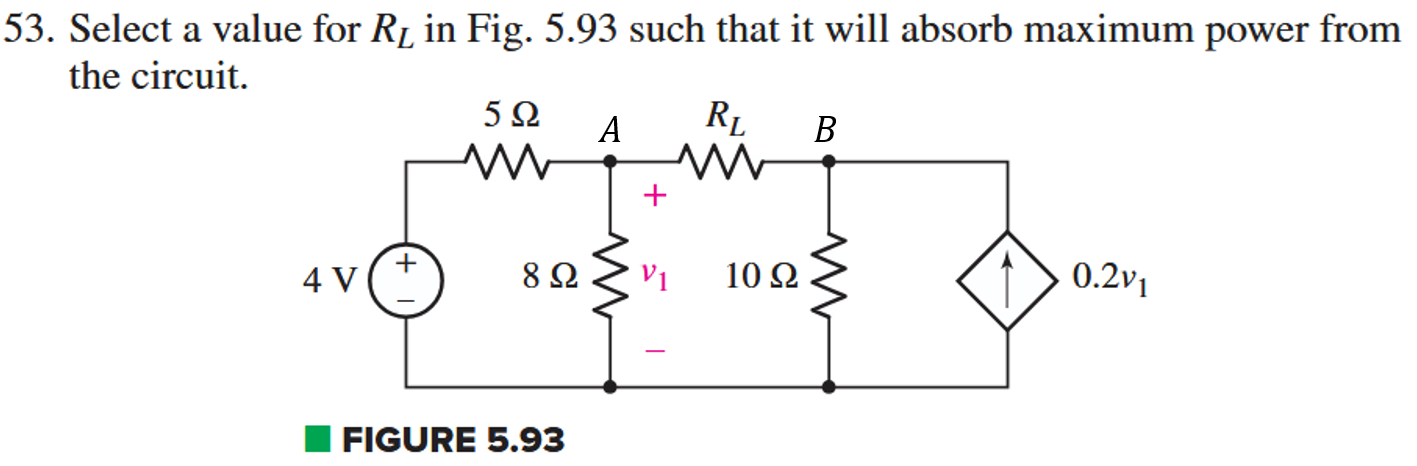
\includegraphics[width=0.8\textwidth]{5-53.png}
\end{center}
\vspace{-1em}
We want to find the Thevenin equivalent resistance. Since there is a dependent source, we either have to find the open circuit voltage $V_{oc}$ and short circuit current $i_{sc}$ or we can apply a test source. We will use the open circuit voltage and short circuit current method.\\\\
Find the voltage at node A by using voltage division:
\[V_A = \frac{[8\,\Omega]}{[5+8\,\Omega]}[4\,\text{V}] = 2.4615\,\text{V}\]
Find the voltage at node B by using Ohms law ($V_1=V_A$):
\[V_B = [10\,\Omega](0.2V_1) = 0.2[10\,\Omega][2.4615\,\text{V}] = 4.923\,\text{V}\]
\[V_{oc} = V_A - V_B = [2.4615\,\text{V}] - [4.923\,\text{V}] = -2.4615\,\text{V}\]
Now we add a short across nodes A and B to find the short circuit current $i_{sc}$:
\begin{center}
    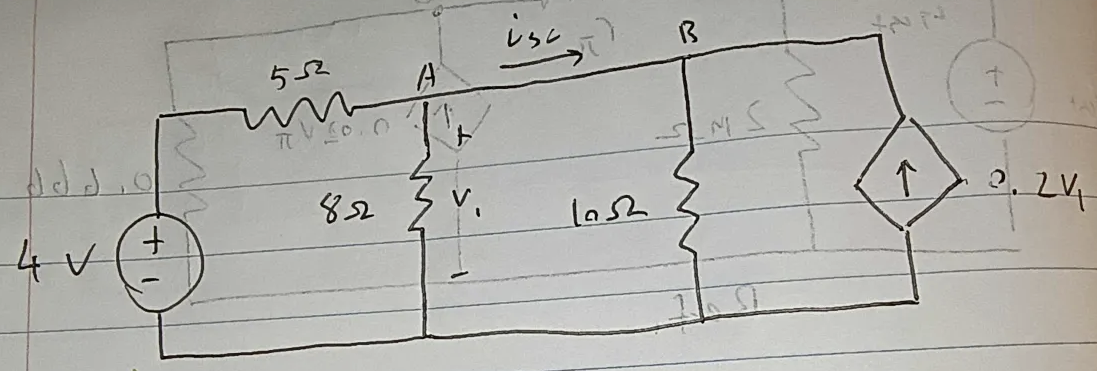
\includegraphics[width=0.8\textwidth]{5-53_1.png}
\end{center}
KCL at node A \& B supernode ($V_1=V_A=V_B$):
\[\frac{4-V_A}{[5\,\Omega]}=\frac{V_A}{[8\,\Omega]}+\frac{V_A}{[10\,\Omega]}-(0.2V_1) \implies V_1 = 3.5555\,\text{V}\]
KCL at node B:
\[i_{sc} = \frac{V_1}{[10\,\Omega]}-(0.2V_1) = \frac{3.5555\,\text{V}}{[10\,\Omega]}-(0.2)(3.5555\,\text{V}) = 0.35555\,\text{A}-(0.7111\,\text{V}) = -0.35555\,\text{A}\]
Thus, the Thevenin equivalent resistance is:
\[R_{Th} = \frac{V_{oc}}{i_{sc}} = \frac{[-2.4615\,\text{V}]}{[-0.35555\,\text{A}]} = \boxed{6.923\,\Omega}\]
The load that absorbs maximum power is when $R_L = R_{Th} = 6.923\,\Omega$.

\section*{5.61}
\vspace{-2em}
\begin{center}
    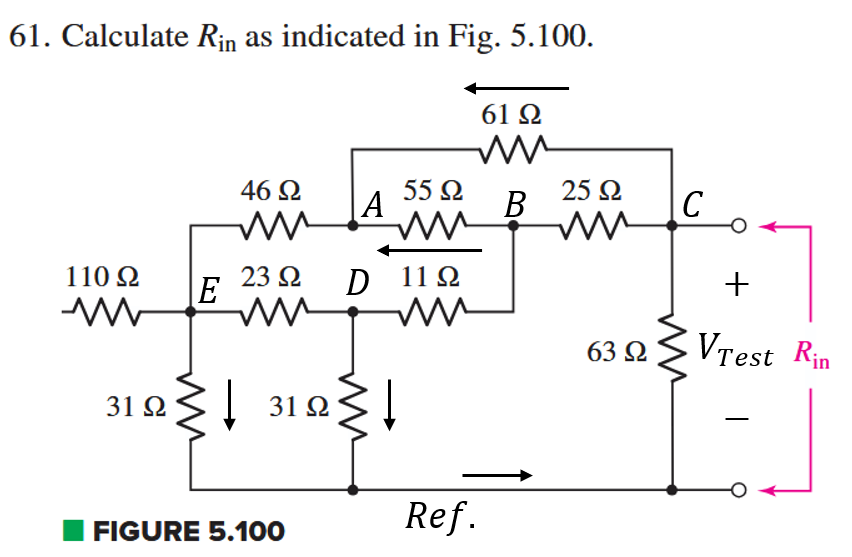
\includegraphics[width=0.8\textwidth]{5-61.png}
\end{center}
\vspace{-1em}
Using a test source $V_{Test} = 1\,\text{V}$, we can find the current $i_{Test}$ and thus the equivalent resistance of the circuit.\\\\
Node A:
\[\frac{V_C-V_A}{[61\,\Omega]}+\frac{V_B-V_A}{[55\,\Omega]}=\frac{V_A-V_E}{[46\,\Omega]}\quad\implies\quad -0.056314V_A+0.01818V_B+0.01639V_C+0.0217V_E=0\]
Node B:
\[\frac{V_C-V_B}{[25\,\Omega]}=\frac{V_B-V_A}{[55\,\Omega]}+\frac{V_B-V_D}{[11\,\Omega]}\quad\implies\quad0.01818V_A - 0.14909V_B + 0.04V_C + 0.09091V_D = 0\]
Node C:
\[V_C = 1\,\text{V}\]
Node D:
\[\frac{V_B-V_D}{[11\,\Omega]}=\frac{V_D-V_E}{[23\,\Omega]}+\frac{V_D}{[31\,\Omega]}\quad\implies\quad0.09091V_B - 0.16665V_D + 0.04348V_E = 0\]
Node E:
\[\frac{V_A-V_E}{[46\,\Omega]}+\frac{V_D-V_E}{[23\,\Omega]}=\frac{V_E}{[31\,\Omega]}\quad\implies\quad0.02174V_A + 0.04348V_D - 0.09748V_E = 0\]
Thus, solving the system of equations: $V_A = 0.6010\,\text{V}$, $V_B = 0.5865\,\text{V}$, $V_C = 1\,\text{V}$, $V_D = 0.4016\,\text{V}$, $V_E = 0.3132\,\text{V}$.\\\\
Thus using KCL at node C:
\[i_\text{Test} = \frac{V_C-V_A}{[61\,\Omega]}+\frac{V_C-V_B}{[25\,\Omega]} + \frac{V_C}{[63\,\Omega]}= 0.03906\,\text{A}\]
Thus, the equivalent resistance of the circuit is:
\[R_{eq} = \frac{V_\text{Test}}{i_\text{Test}} = \frac{1\,\text{V}}{0.03906\,\text{A}} = \boxed{25.599\,\Omega}\]

\section*{6.1}
\vspace{-2em}
\begin{center}
    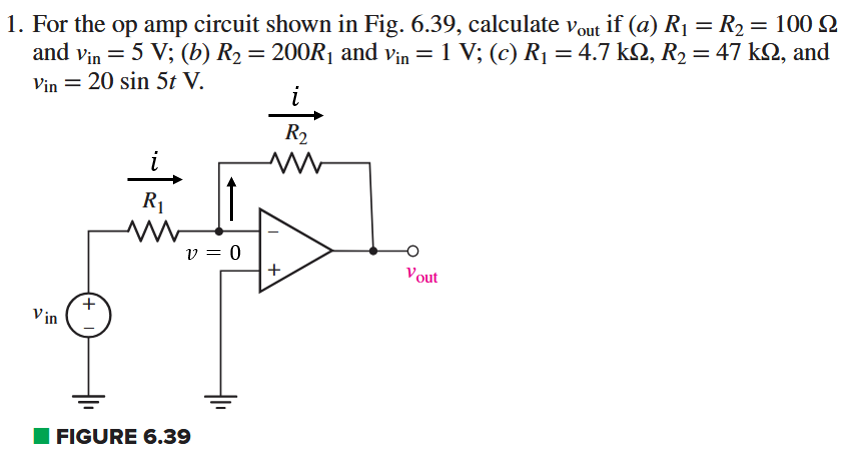
\includegraphics[width=0.8\textwidth]{6-1.png}
\end{center}
\vspace{-1em}
Op-amp rules: No current ever flows into either input terminal. (Current can flow at the output terminal!) There is no voltage difference between the two input terminals. It can either be a source or a sink of current.\\\\
\textbf{(a)} This is an inverting amplifier. We can find the relationship between the input voltage $V_{in}$ and output voltage $V_{out}$ by first using finding the current $i$ by using the fact that the voltage at the inverting terminal is equal to the voltage at the non-inverting terminal (grounded). Thus, the voltage drop over $R_1$ must be equal to $V_\text{in}$:
\[V_\text{in} - R_1 i = 0 \implies i = \frac{V_\text{in}}{R_1}\]
Next, we can sum the voltage drops around the series connection between $R_1$ and $R_2$ to find the relationship between $V_{in}$ and $V_{out}$:
\[V_\text{in} - R_1 i - R_2 i = V_{out} \implies V_{out} = V_\text{in} - (R_1 + R_2)i\]
Substituting the expression for $i$:
\[V_{out} = V_\text{in} - (R_1 + R_2)\frac{V_\text{in}}{R_1} = V_\text{in}\left(1 - \frac{R_1 + R_2}{R_1}\right) = -\frac{R_2}{R_1}V_\text{in}\]
\[\boxed{V_{out} = -\frac{R_2}{R_1}V_\text{in}}\]
Now we just plug in $R_1 = R_2 = 100\,\Omega$, $V_\text{in} = 5\,\text{V}$
\[V_{out} = -\frac{100\,\Omega}{100\,\Omega}[5\,\text{V}] = \boxed{-5\,\text{V}}\]
\textbf{(b)} Plug in $R_2 = 200R_1$, $V_\text{in} = 1\,\text{V}$:
\[V_{out} = -\frac{200R_1}{R_1}[1\,\text{V}] = \boxed{-200\,\text{V}}\]
\textbf{(c)} Plug in $R_1 = 4.7\,\text{k}\Omega$, $R_2 = 47\,\text{k}\Omega$, $V_\text{in} = 20\sin(5t)\,\text{V}$:
\[V_{out} = -\frac{47\,\text{k}\Omega}{4.7\,\text{k}\Omega}[20\sin(5t)\,\text{V}] = \boxed{-200\sin(5t)\,\text{V}}\]

\section*{6.2}
\vspace{-2em}
\begin{center}
    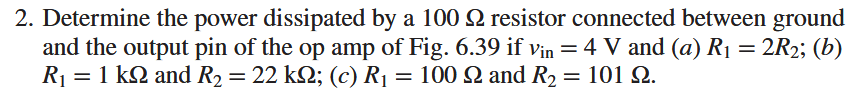
\includegraphics[width=0.8\textwidth]{6-2.png}
\end{center}
\vspace{-2em}
\begin{center}
    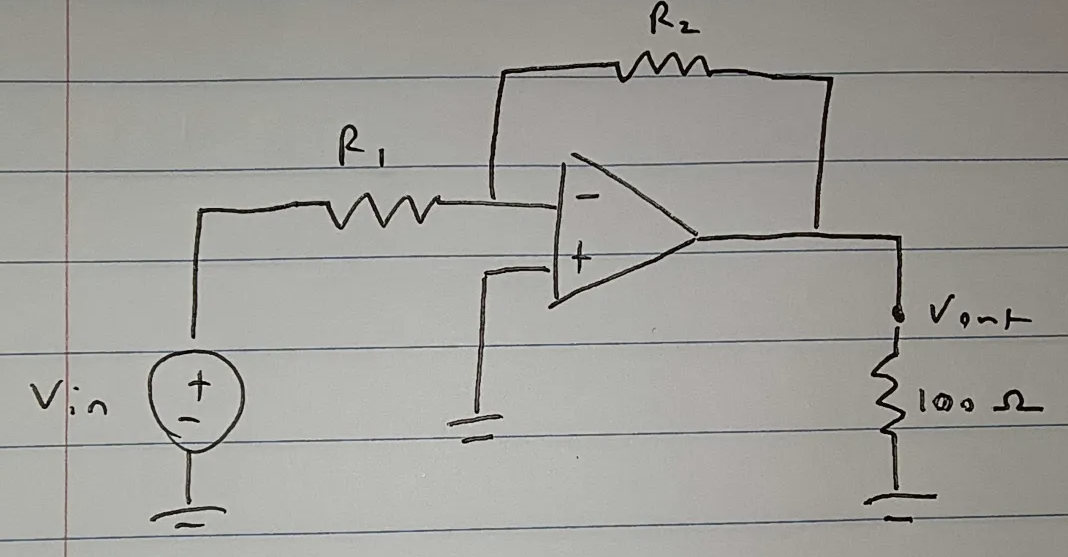
\includegraphics[width=0.6\textwidth]{6-2_1.png}
\end{center}
The voltage across the 100$\Omega$ is the same as $V_\text{out}$ and the power dissipated is given as $P=V^2/R$.\\\\
\textbf{(a)}
\[V_\text{out} = -\frac{R_2}{2R_2}[4\,\text{V}] = -2\,\text{V} \implies P= \frac{(-2\,\text{V})^2}{100\,\Omega} = \boxed{0.04\,\text{W}}\]
\textbf{(b)}
\[V_\text{out} = -\frac{22\,\text{k}\Omega}{1\,\text{k}\Omega}[4\,\text{V}] = -88\,\text{V} \implies P= \frac{(-88\,\text{V})^2}{100\,\Omega} = \boxed{77.44\,\text{W}}\]
\textbf{(c)}
\[V_\text{out} = -\frac{101\,\Omega}{100\,\Omega}[4\,\text{V}] = -4.04\,\text{V} \implies P= \frac{(-4.04\,\text{V})^2}{100\,\Omega} = \boxed{0.1632\,\text{W}}\]

\section*{6.16}
\vspace{-2em}
\begin{center}
    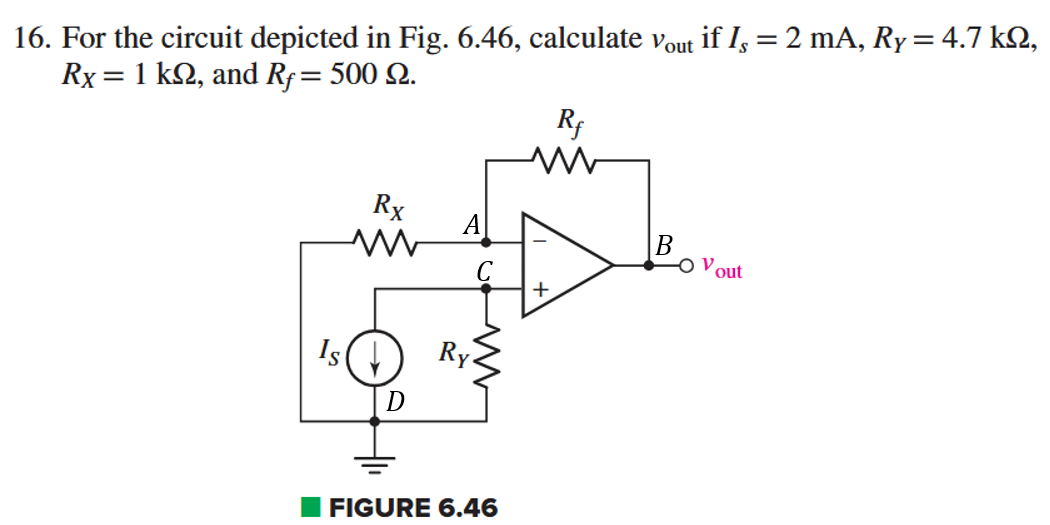
\includegraphics[width=0.8\textwidth]{6-16.png}
\end{center}
\vspace{-1em}
Using KCL at the non-inverting input to find the voltage there:
\[-I_S = \frac{V_{C}}{R_Y} \quad \implies V_{C} = -I_S R_Y = -[2\times10^{-3}\,\text{A}][4.7\times10^3\,\Omega] = -9.4\,\text{V}\]
We can use the rule that the voltage at node A is the same as the voltage at node C to find the output voltage using KCL at node A (sum of current entering node A is zero, since it is an input terminal):
\[V_C=V_A\]
\[\frac{0-V_A}{R_X} + \frac{V_A-V_\text{out}}{R_f} = 0 \quad\implies V_\text{out} = V_A\left(1 + \frac{R_f}{R_X}\right)\]
\[\boxed{V_\text{out} = [-9.4\,\text{V}]\left(1 + \frac{[500\,\Omega]}{[1\times10^3\,\Omega]}\right) = -14.1\,\text{V}}\]

\section*{6.20}
\vspace{-2em}
\begin{center}
    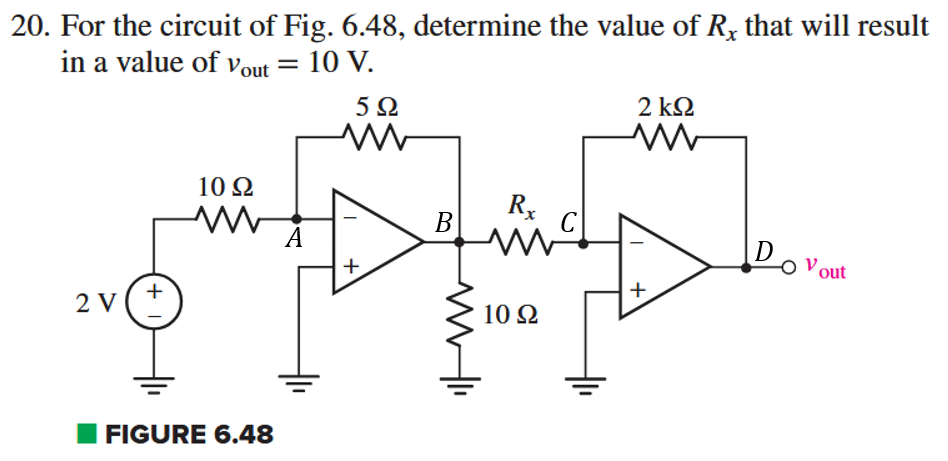
\includegraphics[width=0.8\textwidth]{6-20.png}
\end{center}
\vspace{-1em}
Since the op-amp on the left is an inverting amplifier, we can find the output voltage at node B using the equation:
\[V_\text{out} = -\frac{R_2}{R_1}V_\text{in}\implies V_B = -\frac{[5\,\Omega]}{[10\,\Omega]}[2\,\text{V}] = -1\,\text{V}\]
We know that the voltage at node C is zero since the non-inverting input is grounded. Thus, we can use KCL at node C to find the output voltage in terms of $R_x$:
\[\frac{V_C-V_B}{R_x}=\frac{V_\text{out}-V_C}{[2\,\text{k}\Omega]} \implies R_x = -\frac{V_B}{V_\text{out}} \cdot [2\,\text{k}\Omega]=-\frac{[-1\,\text{V}]}{[10\,\text{V}]}[2\,\text{k}\Omega]=\boxed{0.2\,\text{k}\Omega}\]

\section*{6.25}
\vspace{-2em}
\begin{center}
    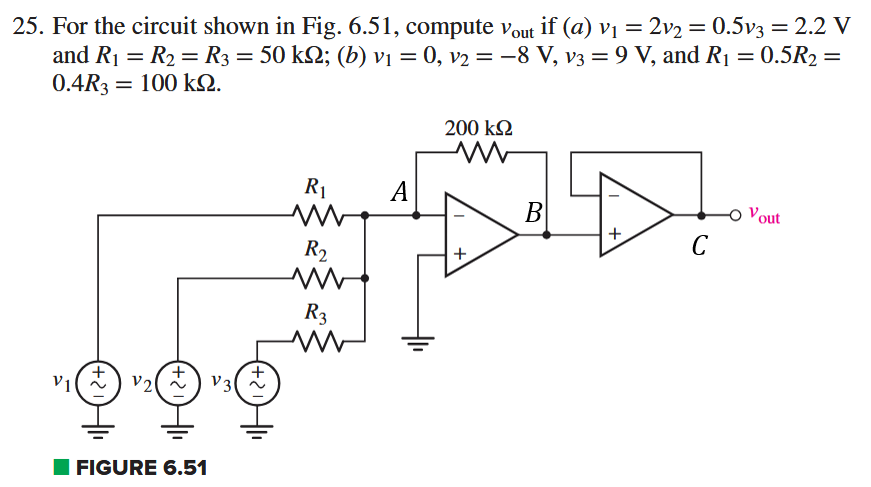
\includegraphics[width=0.8\textwidth]{6-25.png}
\end{center}
\vspace{-1em}
The op-amp on the left is an inverting summer circuit. The op-amp on the right is a buffer circuit. Thus, we can use the equations for a summer circuit to find the output voltage at node B:
\[V_o = -\left(\frac{R_f}{R_1}V_1 + \frac{R_f}{R_2}V_2 + \frac{R_f}{R_3}V_3\right) \implies V_B = -\left(\frac{[200\,\text{k}\Omega]}{[R_1]}V_1 + \frac{[200\,\text{k}\Omega]}{R_2}V_2 + \frac{[200\,\text{k}\Omega]}{R_3}V_3\right)\]
The equation for a buffer circuit is
\[V_\text{out} = V_\text{in}\]
Thus, the output voltage is:
\[V_\text{out} = V_B = -\left(\frac{[200\,\text{k}\Omega]}{[R_1]}V_1 + \frac{[200\,\text{k}\Omega]}{R_2}V_2 + \frac{[200\,\text{k}\Omega]}{R_3}V_3\right)\]
\textbf{(a)} Plugging in $V_1=2V_2=0.5V_3 = 2.2\,\text{V} \implies$ $V_2 = 1.1\,\text{V}$, $V_3 = 4.4\,\text{V}$ and $R_1 = R_2 = R_3 = 50\,\text{k}\Omega$:
\[V_\text{out} = -\left(\frac{[200\,\text{k}\Omega]}{[50\,\text{k}\Omega]}[2.2\,\text{V}] + \frac{[200\,\text{k}\Omega]}{[50\,\text{k}\Omega]}[1.1\,\text{V}] + \frac{[200\,\text{k}\Omega]}{[50\,\text{k}\Omega]}[4.4\,\text{V}]\right) = \boxed{-30.8\,\text{V}}\]
\textbf{(b)} Plugging in $V_1=0$, $V_2=-8\,\text{V}$, $V_3=9\,\text{V}$ and $R_1 = 0.5R_2 = 0.4R_3=100\,\text{k}\Omega \implies$ $R_2 = 200\,\text{k}\Omega$, $R_3 = 250\,\text{k}\Omega$:
\[V_\text{out} = -\left(\frac{[200\,\text{k}\Omega]}{[100\,\text{k}\Omega]}[0] + \frac{[200\,\text{k}\Omega]}{[200\,\text{k}\Omega]}[-8\,\text{V}] + \frac{[200\,\text{k}\Omega]}{[250\,\text{k}\Omega]}[9\,\text{V}]\right) = \boxed{0.8\,\text{V}}\]

\section*{6.33}
\vspace{-2em}
\begin{center}
    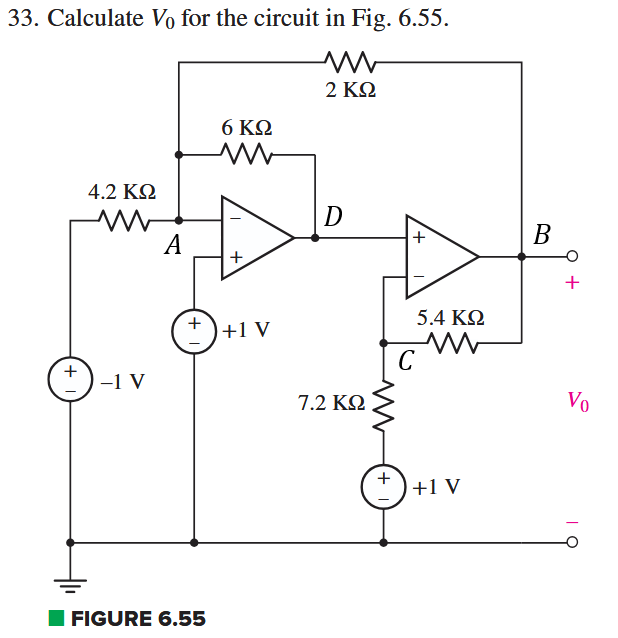
\includegraphics[width=0.6\textwidth]{6-33.png}
\end{center}
\vspace{-1em}
Sadly we will need to do nodal analysis to find the output voltage. Starting with the left op-amp, the voltage at node A is 1 V since the non-inverting input is 1 V.\\\\
Using KCL at node A ($V_A = 1$ V):
\[\frac{[-1\,\text{V}]-V_A}{[4.2\,\text{k}\Omega]}=\frac{V_A-V_D}{[6\,\text{k}\Omega]}+\frac{V_A-V_B}{[2\,\text{k}\Omega]}\implies 0.90476V_A-0.5V_B-0.16666V_D = -0.238095\]
To find $V_D$ we can use KCL at node C ($V_C=V_D$):
\[\frac{V_B-V_C}{[5.4\,\text{k}\Omega]}=\frac{V_C-[1\,\text{V}]}{[7.2\,\text{k}\Omega]}\implies 0.185185V_B-0.324074V_D=-0.138888\]
Thus, $V_B = 1.8000\,\text{V}$ and $V_D = 1.4571\,\text{V}$.\\\\
The output voltage is the same as the voltage at node B, so \[\boxed{V_\text{out} = V_B = 1.8\,\text{V}}\]
\underline{Note:} The -1V source makes it a bit trippy but stick with convention that there is a voltage drop across the 4.2 k$\Omega$ resistor along the direction of current, thus the potential difference is $(-1\,\text{V})-V_A$.

\section*{6.56}
\vspace{-2em}
\begin{center}
    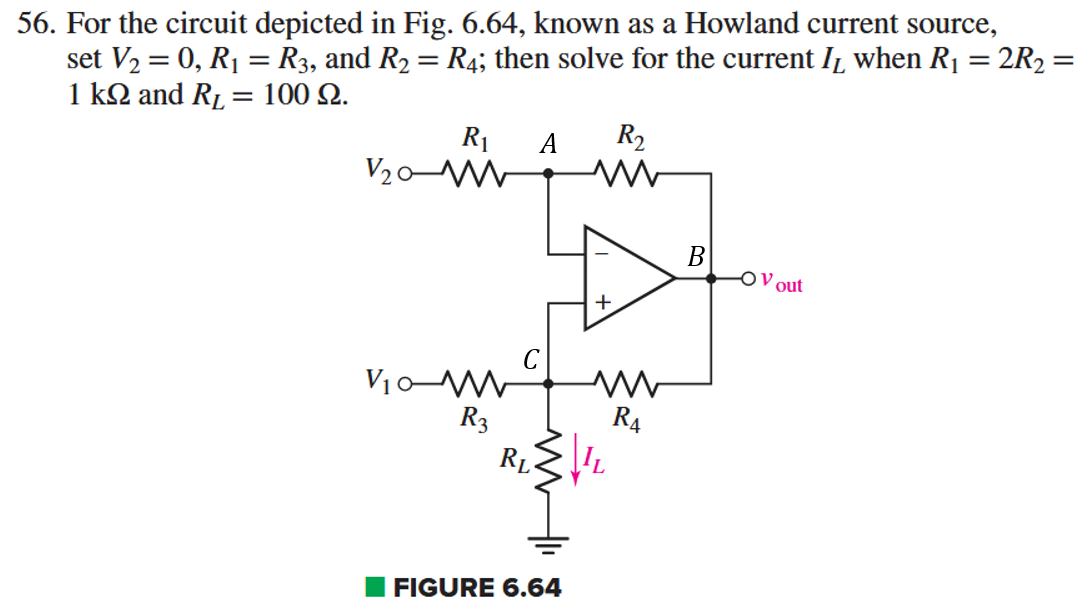
\includegraphics[width=0.8\textwidth]{6-56.png}
\end{center}
\vspace{-1em}
Given $V_2 = 0$ V and $R_1 = 1\,\text{k}\Omega$, $R_2 = 0.5\,\text{k}\Omega$, $R_3 = 1\,\text{k}\Omega$, $R_4 = 0.5\,\text{k}\Omega$, $R_L = 0.1\,\text{k}\Omega$., we can write the following nodal equations:
\[V_A=V_C\]
Node A:
\[\frac{V_2-V_A}{R_1} = \frac{V_A-V_B}{R_2}\implies V_C\left(\frac{1}{R_2}+\frac{1}{R_1}\right)-\frac{V_B}{R_2} = 0\implies V_B =1.5V_C \]
Node C:
\[\frac{V_B-V_C}{R_4}=\frac{V_C-V_1}{R_3}+\frac{V_C}{R_L}\implies \frac{V_B}{R_4} -V_C\left(\frac{1}{R_4}+\frac{1}{R_3}+\frac{1}{R_L}\right) = -\frac{V_1}{R_3}\]
Substituting $V_B$ into the equation for node C and plugging in the values for the resistors:
\[3V_C-13V_C=-V_1 \implies V_C = \frac{V_1}{10}\]
Thus the current $I_L$ is:
\[I_L = \frac{V_C}{R_L} = \frac{V_1/10}{[100\,\Omega]} = \boxed{0.001V_1}\]
\end{document}